% !TeX program = xelatex
% !TeX encoding = UTF-8
\documentclass[conference,a4paper]{IEEEtran}

% ICSMD 2026: A4, two-column IEEE conference layout, 5--6 pages.
\usepackage{fontspec}
\setmainfont{Times New Roman}
\setsansfont{Arial}
\setmonofont{Consolas}

\usepackage{amsmath,amssymb}
\usepackage{graphicx}
\usepackage{booktabs}
\usepackage{array}
\usepackage{tabularx}
\usepackage{multirow}
\usepackage{url}
\usepackage{xurl}
\usepackage{cite}
\usepackage{pgfplots}
\usepackage{balance}
\usepackage{float}
\usepackage{microtype}
\pgfplotsset{compat=1.18}

\IEEEoverridecommandlockouts

\setlength{\columnsep}{0.24in}
\setlength{\textfloatsep}{5pt plus 1pt minus 1pt}
\setlength{\floatsep}{4pt plus 1pt minus 1pt}
\setlength{\intextsep}{4pt plus 1pt minus 1pt}
\setlength{\abovecaptionskip}{3pt}
\setlength{\belowcaptionskip}{0pt}
\renewcommand{\arraystretch}{1.08}

\title{Evidence-Traceable Knowledge Graph Construction from Marine Pump Technical Documents via Automated Evidence-Quality Gating}

\author{%
\IEEEauthorblockN{Xiaokun Zhang\textsuperscript{1}, Dongliang Fu\textsuperscript{1,*}, Rui Wang\textsuperscript{2}, and Erwu Liu\textsuperscript{2}}
\IEEEauthorblockA{\textsuperscript{1}Shanghai Marine Equipment Research Institute (SMERI), China State Shipbuilding Corporation (CSSC), Shanghai, China\\
\textsuperscript{2}Tongji University, Shanghai, China\\
\textsuperscript{*}Corresponding author: Dongliang Fu; e-mail: fdl@163.com}}

\begin{document}
\maketitle

\begin{abstract}
Measurements from marine engine-room pumps become more interpretable and auditable when linked to documented causes, inspections, and maintenance actions. Large language models can extract such relations from manuals, but their outputs may contain unlocatable evidence, reversed relations, misaligned table cells, or duplicated support copied across documents. This paper presents an automated evidence-quality gating method for constructing a page-traceable and auditable knowledge graph. Each normalized triple is stored separately from every page-level evidence record that supports it. Admission requires valid graph structure and direction, recoverable page or table evidence, relation support, complete provenance, build-corpus membership, and non-inference. A full audit graph retains all candidates and gate outcomes; evidence-qualified records with normalized Chinese terminology form tiered application graphs. From 15 documents and 1,934 physical pages, the pipeline produced 8,003 audit records, of which 1,698 passed all evidence gates. The standard application layer contains 1,326 evidence records, 1,281 unique triples, and 2,022 Chinese entities, covering 78.09\% of the qualified set. All qualified records passed a label-blind re-localization and provenance audit, and all 13,729 controlled rule violations triggered at least one gate. In four held-out documents from one source family, 81 records met the non-corpus evidence gates with complete page localization and provenance but remained outside the application graph. Eightfold replication within one source family did not change the family-capped support score. The method enables evidence-grounded graph construction without manual approval of every triple at admission time. Qualification denotes compliance with declared evidence rules, not expert-confirmed factual or diagnostic accuracy.
\end{abstract}

\begin{IEEEkeywords}
marine pump systems, knowledge graph, evidence-quality gating, page-level provenance, terminology normalization, condition-monitoring knowledge
\end{IEEEkeywords}

\section{Introduction}

Pumps, motors, pipes, and valves in a ship's engine room support cooling, ballast transfer, bilge drainage, and fuel delivery. Condition-monitoring systems observe insufficient inlet pressure, reduced flow, elevated vibration, high temperature, and abnormal current \cite{ABS2016,ABS2023}. These measurements seldom identify a fault alone; engineers consult classification guidance, manuals, and maintenance tables to link them to possible causes and actions.

Such knowledge is evidence-dependent. A relation may appear in prose, a troubleshooting table, or a maintenance procedure; tables may contain merged rows and inherited headers. Retaining only a deduplicated head--relation--tail triple loses the exact supporting passage. Moreover, manuals from one source often repeat content, so document count overstates independent support.

Knowledge graphs organize equipment, faults, symptoms, inspections, and maintenance actions \cite{Hogan2021,Ji2022}. LLMs reduce extraction effort, but schema alignment, canonicalization, and output stability still require explicit controls \cite{Zhang2024EDC}. Industrial fault graphs mainly address extraction, fusion, reasoning, or diagnosis \cite{Han2022,Cai2024,Wu2024}. A preceding issue remains: what document-evidence conditions should an automatically extracted record satisfy before entering an application graph?

We treat each generated triple as a candidate, not a fact. It must point to recoverable evidence and pass frozen executable checks for field completeness, structure, direction, localization, provenance, and corpus boundaries. Passing denotes compliance with these admission rules, not expert confirmation of objective truth.

The study asks whether the pipeline produces schema-compliant, page-localized, provenance-complete records (RQ1); how evidence and terminology gates affect filtering, graph size, and cost (RQ2); whether frozen rules transfer to held-out sources (RQ3); whether source-family capping resists within-family duplication (RQ4); and how terminology tiers affect predefined fault-path coverage and density (RQ5).

The contributions are threefold. First, normalized triples are separated from page-level evidence records, preserving multiple supports after semantic deduplication. Second, executable gates jointly determine qualification, quarantine, or rejection and retain a complete audit trail. Third, tiered Chinese application graphs are derived from the audit graph, while source-family capping limits repeated documents assigned to one family from appearing as independent corroboration. We evaluate these mechanisms by complete-candidate re-audit, controlled fault injection, terminology sensitivity, source holdout, and replication stress tests.

\section{Related Work}

\subsection{LLM-Based Knowledge Graph Construction}

Knowledge graph construction combines extraction, schema alignment, canonicalization, and fusion \cite{Hogan2021,Ji2022}. Extract-Define-Canonicalize separates open extraction, schema definition, and post-hoc canonicalization, showing why LLM construction is not a single prompting step \cite{Zhang2024EDC}. Industrial graphs support process monitoring, rotating machinery, and equipment diagnosis \cite{Han2022,Cai2024,Wu2024}. Our focus is earlier: the evidence requirements that generated records must meet when manual review of every triple is not a prerequisite.

\subsection{Statement-Level Provenance and Evidence Support}

W3C PROV-O represents derivation through entities, activities, and agents \cite{W3CPROVO}; named or contextualized graphs can retain statement-level provenance \cite{Sikos2020}. RDF 1.2 triple terms and reifiers describe a statement without directly asserting it \cite{W3CRDF12}, while nanopublications separate an assertion from provenance and publication information \cite{Groth2010}. ProVe verifies textual support for graph triples \cite{Amaral2024ProVe}; SciGraph-LLM jointly extracts atomic claims, source spans, and provenance \cite{Malashin2026}.

Marine documents add physical-page and table localization, directed relations, Chinese terminology, and repeated content within source families. Rather than proposing a provenance standard, we turn established representation principles into an executable admission workflow.

\section{Method}

\subsection{Corpus Partition and Page Parsing}

MP numbers are corpus registry IDs, not a continuous build-set sequence. The build set comprises MP001--MP007 and MP015--MP022: 15 documents and 1,934 physical pages. MP008 was used for development, MP009 for a preliminary non-blind transfer check, and MP010--MP013 for source-held-out evaluation after freezing the method and primary graph; none entered that graph. MP014 was excluded because it is an offshore electric-submersible-pump signal dataset rather than a marine technical document.

Deterministic rules removed blank, cover/title, contents, index, and exact-duplicate pages, leaving 1,889 extraction pages. Each page object retained text, table cells, bounding boxes, physical page, URL, publisher, source family, and document/page hashes. Candidate generation used the Alibaba Cloud Model Studio alias \mbox{qwen3.7-max} through the DashScope API at temperature zero on July 26--27, 2026; requests and responses were cached. The API records contain the alias rather than a dated model snapshot, so the historical backend snapshot cannot be established retrospectively.

The schema contains 13 node and 15 relation types. Allowed endpoint types, relation directions, the whitelist, terminology dictionary, source-family assignments, and thresholds were frozen before full-corpus construction. Domain knowledge was thus encoded in reusable rules rather than ad hoc admission decisions.

\subsection{Normalized Triples and Page-Level Evidence Records}

A normalized triple is denoted by
\begin{equation}
c_i=(h_i,r_i,t_i),
\label{eq:triple}
\end{equation}
where $h_i$, $r_i$, and $t_i$ are the head entity, relation, and tail entity. Every occurrence of document support creates a separate page-level evidence record:
\begin{equation}
a_i=\langle c_i,e_i,p_i,g_i\rangle,
\label{eq:evidence}
\end{equation}
where $e_i$ stores the verbatim passage and page span or table cell, $p_i$ stores provenance, and $g_i$ stores evidence type, support mode, score, and gate outcomes. A triple may link to multiple evidence records; semantic deduplication never overwrites page-level support.

For example, MP016 p.~3 states that insufficient inlet pressure causes pump cavitation. The model proposes \emph{insufficient inlet pressure--causes--cavitation}. The system validates its types and direction, relocates both endpoints and the relation phrase, and stores page, URL, hashes, and source family. A repeated sentence in another manual adds evidence but not another contribution from that family.

\subsection{Automated Evidence-Quality Gating}

The gates comprise four groups.

\textbf{Structure:} Endpoint types, relation, and direction must comply with the whitelist and schema.

\textbf{Evidence:} E1 requires both entities in one continuous page span. E2 requires relevant cells in one row or validated merged-row group, preserving cell IDs and bounding boxes. Cross-sentence E3 records remain auditable but cannot enter an application graph.

\textbf{Relation support:} Explicit rules require an unambiguous phrase or table role. Otherwise, the extraction model receives support- and rejection-oriented prompts. Both must support the relation at confidence $\geq0.9$, with relocatable quotations.

\textbf{Admission boundary:} The governance score $q_i=\alpha_i w_E(l_i)w_R(\eta_i)$ combines model-reported confidence $\alpha_i$ with frozen weights for evidence level and relation-support status. The weights for E1/E2/E3 are 1.00/0.95/0.75, and those for supported/undetermined/unsupported relations are 1.00/0.75/0. A record must belong to the build set, be non-inferred, contain complete URL/family/hash provenance, and have $q_i\geq0.8$. This heuristic supports filtering; it is not a factual probability.

The combined gate is
\begin{equation}
H(a_i)=I_{str}I_{dir}I_{loc}I_{sup}I_{prov}I_{build}I_{noninf}I_{q\geq0.8}.
\label{eq:gate}
\end{equation}
All indicators must equal one. Unresolved relations, E3 evidence, and other recoverable cases are quarantined; unlocatable, structurally invalid, or unsupported records are rejected.

\begin{figure*}[t]
  \centering
  \IfFileExists{RP1_ICSMD2026_method_flowchart_en.pdf}{%
    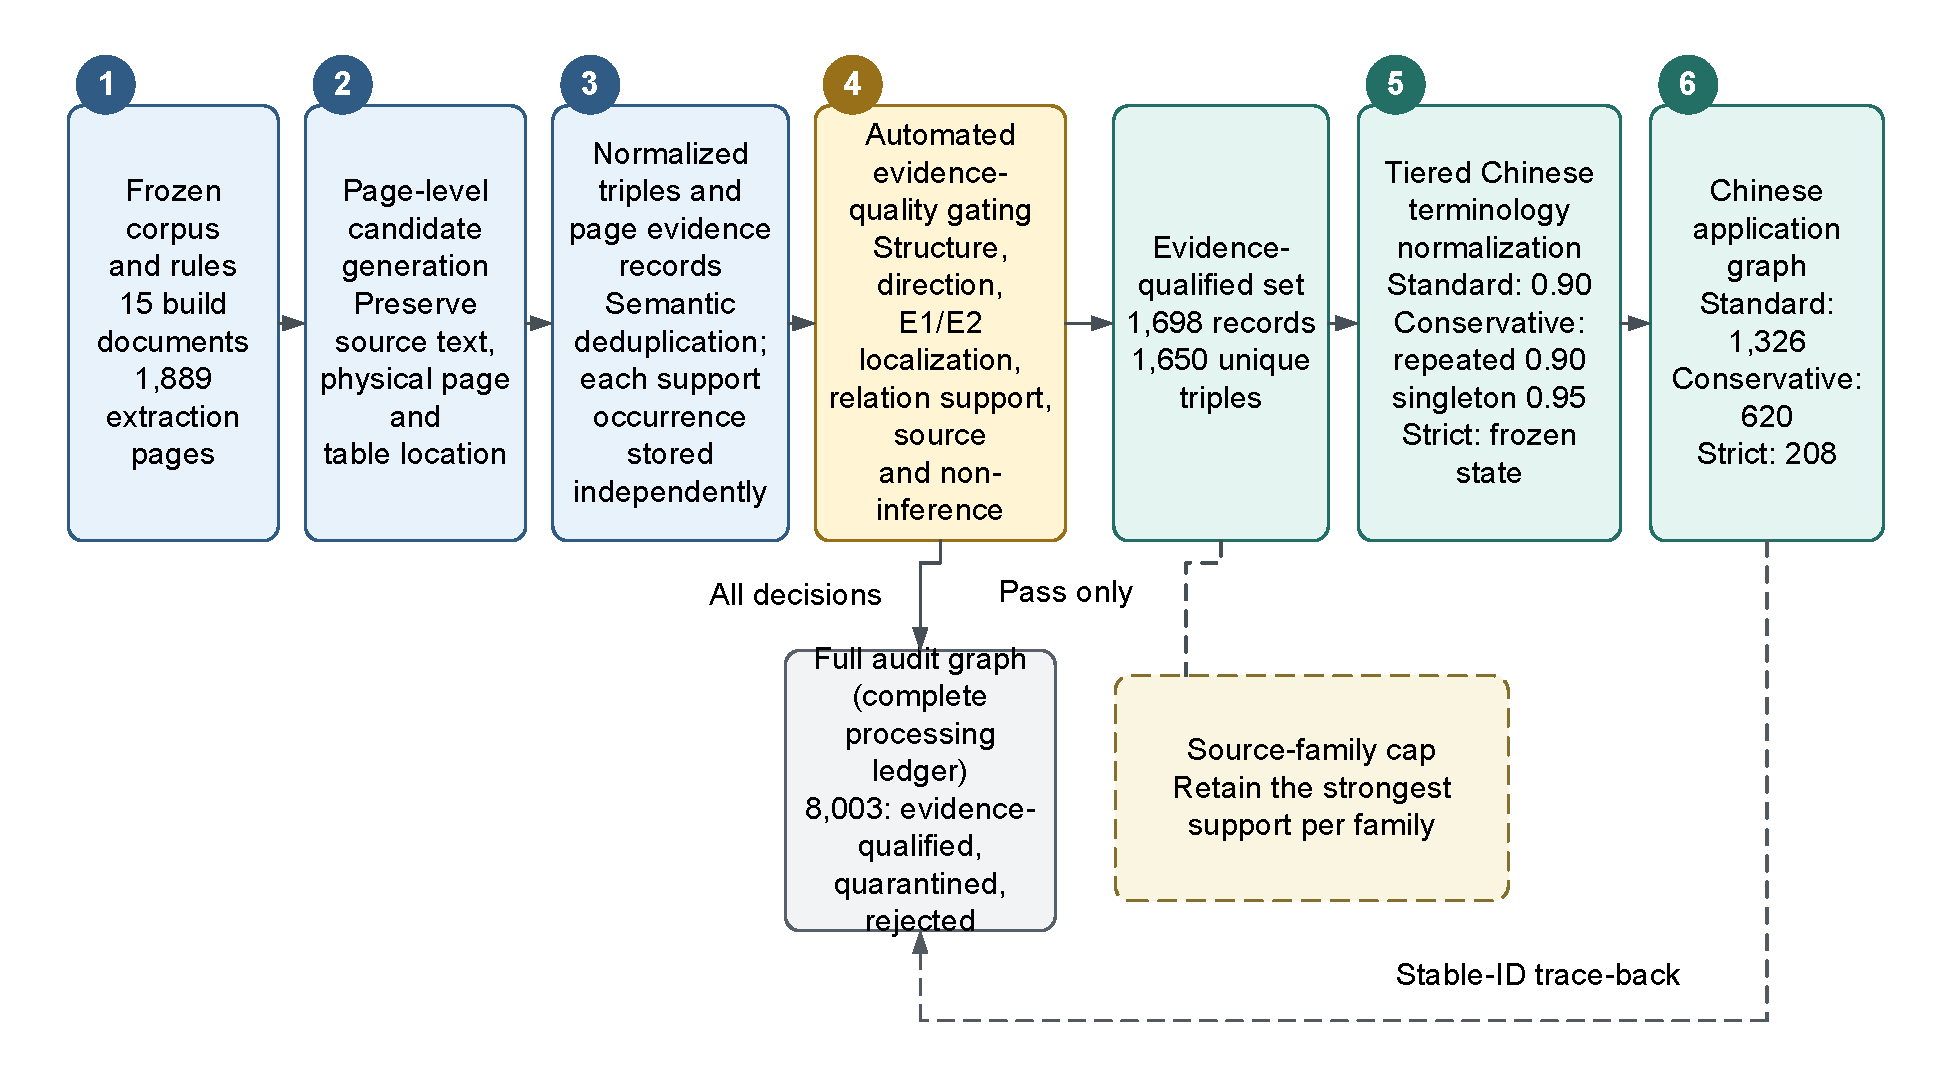
\includegraphics[width=0.90\textwidth]{RP1_ICSMD2026_method_flowchart_en.pdf}%
  }{\fbox{\parbox[c][35mm][c]{0.94\textwidth}{\centering Export the English workflow from the Visio source in this directory.}}}
  \caption{Workflow for automated evidence-quality gating, the complete processing ledger, and tiered Chinese application graphs.}
  \label{fig:pipeline}
\end{figure*}

\subsection{Full Audit Graph and Tiered Chinese Application Graphs}

The \emph{full audit graph} retains every candidate, gate outcome, and failure reason. The \emph{Chinese application graph} selects qualified, non-inferred records for retrieval and visualization, then assigns standard, conservative, or strict layers from both endpoints' terminology status. Stable IDs link each application record to the audit graph and physical page (Fig.~\ref{fig:pipeline}).

Normalization never rewrites verbatim evidence. Frozen dictionary and earlier two-prompt terms are retained. Other Chinese names require completeness, no same-type naming conflict, protected-string preservation, and the layer threshold. Standard uses 0.90; conservative uses 0.90 for recurring endpoints and 0.95 for singletons; strict retains only the original frozen status. Protected strings include models, units, API, ISO, and NPSH. These checks indicate local consistency, not independent or expert confirmation.

\subsection{Source-Family Capping}

Manuals from one publisher may share content. For triple $c$, only the strongest evidence score in each publisher- or document-defined family is retained:
\begin{equation}
s_f(c)=\max_{a_i\in A_f(c)}q_i,\quad
S_{fam}^{(B)}(c)=\frac{1}{B}\sum_{j=1}^{\min(B,|F_c|)}s_{(j)}(c).
\label{eq:family}
\end{equation}
Here $F_c$ is the set of families supporting $c$, $s_{(j)}$ is the $j$th-largest family score, and $B=2$ is the frozen engineering coverage target; missing family slots contribute zero. The index is audit and ranking metadata and does not change gate decisions or application-graph membership. Duplicates within one family therefore cannot increase its contribution. The family label is an engineering proxy for dependence, not proof of independence.

\section{Experiments and Results}

\subsection{Experimental Setup}

Evaluation covered full-corpus gating; candidate re-audit; controlled fault injection; prompt-rule cost on fixed pages; terminology layers; and source holdout, within-family replication, and fault paths. Audit, fault-injection, and terminology experiments ran locally without human factual labels, and the terminology experiment sent no passages to an external model. Manifests recorded SHA-256 hashes of candidates, schema, and page files.

\begin{table}[t]
\caption{Page Localization and Provenance Re-Audit}
\label{tab:audit}
\centering
\footnotesize
\setlength{\tabcolsep}{3.2pt}
\begin{tabular}{lrrrr}
\toprule
Decision & Records & Evidence & Endpoints & Subchecks \\
\midrule
Qualified   & 1698 & 100.00\% & 100.00\% & 100.00\% \\
Quarantined & 881  & 100.00\% & 100.00\% & 62.54\% \\
Rejected    & 5424 & 72.77\%  & 48.80\%  & 31.47\% \\
\bottomrule
\end{tabular}
\end{table}

\begin{table}[t]
\caption{Controlled Fault-Injection Results}
\label{tab:mutation}
\centering
\footnotesize
\setlength{\tabcolsep}{3.0pt}
\begin{tabular}{llrr}
\toprule
Fault group & Corrupted fields & Cases & Detection \\
\midrule
Identity/provenance & hash, URL, family & 6792 & 100.00\% \\
Page/evidence       & page, span, endpoints & 4943 & 100.00\% \\
Structural type     & relation-tail type & 1698 & 100.00\% \\
Table structure     & cell ID, bounding box & 296 & 100.00\% \\
\midrule
Total & 10 fault types & 13729 & 100.00\% \\
\bottomrule
\end{tabular}
\end{table}

\begin{table*}[!t]
\caption{Effect of Chinese Terminology Layers on Application-Graph Size and Fault-Path Density}
\label{tab:tiers}
\centering
\footnotesize
\setlength{\tabcolsep}{3.5pt}
\begin{tabularx}{\textwidth}{l>{\raggedright\arraybackslash}Xrrrrrr}
\toprule
Layer & Terminology rule & Evidence & Unique & Chinese & Path & Mean & Mean \\
      &                  & records  & triples & entities & coverage & answers & evidence \\
\midrule
Strict & Frozen dictionary and two-prompt status & 208  & 203  & 281  & 34/40 & 5.075 & 6.150 \\
Conservative & Recurring 0.90; singleton 0.95 & 620  & 590  & 870  & 34/40 & 5.575 & 6.800 \\
Standard & Uniform threshold of 0.90 & 1326 & 1281 & 2022 & 34/40 & 6.400 & 7.700 \\
\bottomrule
\end{tabularx}
\end{table*}

\begin{table}[!t]
\caption{Prompt Rules and Token Cost on Fixed Pages}
\label{tab:prompt}
\centering
\footnotesize
\setlength{\tabcolsep}{2.7pt}
\begin{tabular}{lrrrrr}
\toprule
Method & Raw & Qual. & Qual./raw & Tok./qual. & Qual./100k \\
\midrule
B0   & 162 & 0   & 0.00\%  & --     & 0.0 \\
B1   & 312 & 50  & 16.03\% & 3565.3 & 28.0 \\
B2   & 226 & 31  & 13.72\% & 5238.0 & 19.1 \\
B3   & 254 & 32  & 12.60\% & 5329.8 & 18.8 \\
Ours & 367 & 148 & 40.33\% & 1466.7 & 68.2 \\
\bottomrule
\end{tabular}
\end{table}

\subsection{Complete Candidate Re-Audit and Controlled Fault Injection}

The 8,003 records referenced 922 physical pages. Without reading original decision labels, re-audit reloaded page objects and checked document-page mappings, hashes, URLs, publishers, families, evidence and endpoint spans, and E2 table locations.

Table~\ref{tab:audit} shows that all 1,698 qualified records passed localization, provenance, and type checks. All 881 quarantined records retained locatable evidence and endpoints; 330 failed the listed subchecks because they used E3 reconstruction. Of 5,424 rejected records, 3,947 retained locatable evidence, 2,647 both endpoints, and 1,707 all listed subchecks. Rejection may instead reflect relation support, score, or another gate: localization is necessary, not sufficient.

Fault injection corrupted one declared rule at a time in the 1,698 qualified records. Ten fault types covered identity/provenance, page/evidence location, endpoint types, and tables. Every valid mutation triggered a gate (Table~\ref{tab:mutation}); this tests encoded-rule response, not general semantic-error detection.

\subsection{Full-Corpus Graph, Terminology Layers, and Gate Contributions}

From 8,071 raw candidates, normalization and deduplication produced 8,003 audit records: 1,698 qualified, 881 quarantined, and 5,424 rejected. Qualified records represent 1,650 unique triples and 2,613 source-language entities.

By relation-support mode, explicit phrases supported 784 records and table roles supported 98; the other 816 used same-model two-prompt consistency and were marked separately because it is not independent validation. By evidence-localization mode, the qualified set comprised 1,550 E1 and 148 E2 records.

Sequential gates removed 1,292 records by schema/type, 4,206 by E1/E2 localization, 801 by relation support, and six by the 0.8 score. Extending terminology processing moved 1,118 of 1,490 strict-layer exclusions into the standard layer without changing evidence decisions or provenance.

Terminology processing held all 1,698 evidence decisions fixed (Table~\ref{tab:tiers}). The standard layer covers 78.09\% and, versus strict, adds 1,118 records, 1,078 triples, and 1,741 Chinese entities, yielding 6.38 times as many records. The remaining 372 lacked complete, conflict-free, sufficiently confident names or failed protected-string-preservation checks. A repeated-form-only rule at 0.90 yields 237 records, 216 triples, and 301 entities.

Across 36 custom Python release checks---covering file integrity, stable-ID uniqueness, evidence-link closure, split isolation, E1/E2 and non-inference, provenance, relation domain/range, terminology admission, and verbatim immutability---no release-blocking violation was found for the standard or conservative layer. One non-blocking warning concerned 40 rejected records without verbatim text. The 0.80 evidence threshold controls qualification; 0.90/0.95 terminology thresholds control application-layer membership.

Raising the evidence threshold from 0.80 to 0.85, 0.90, 0.925, 0.95, and 0.975 reduced qualification from 1,698 to 1,678, 1,525, 895, 867, and 36 (Fig.~\ref{fig:threshold}). At 0.975, the remaining 36 records spanned eight of the ten predefined fault classes. The frozen 0.80 is an engineering tradeoff, not fitted to human labels.

\begin{figure}[t]
\centering
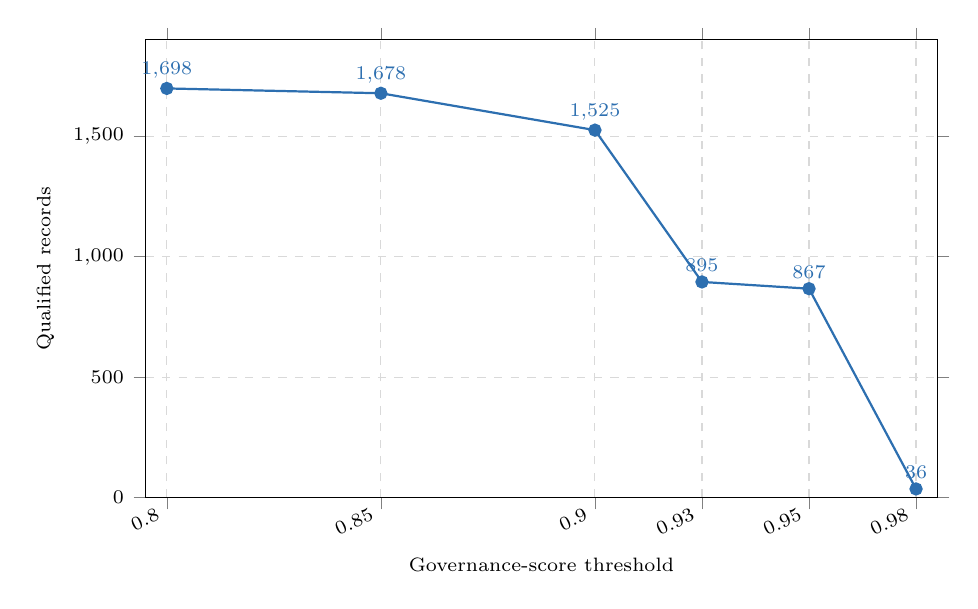
\begin{tikzpicture}
\begin{axis}[
  width=0.96\columnwidth,
  height=0.61\columnwidth,
  xlabel={Governance-score threshold},
  ylabel={Qualified records},
  xmin=0.795, xmax=0.980,
  ymin=0, ymax=1900,
  xtick={0.800,0.850,0.900,0.925,0.950,0.975},
  xticklabel style={font=\scriptsize,rotate=25,anchor=east},
  yticklabel style={font=\scriptsize},
  label style={font=\scriptsize},
  grid=major,
  grid style={draw=gray!30,dashed},
  axis line style={black},
  tick align=outside,
  nodes near coords,
  every node near coord/.append style={font=\scriptsize,anchor=south},
]
\addplot[color={rgb,255:red,45;green,111;blue,176},mark=*,thick]
coordinates {(0.800,1698) (0.850,1678) (0.900,1525) (0.925,895) (0.950,867) (0.975,36)};
\end{axis}
\end{tikzpicture}
\caption{Effect of the governance-score threshold on the number of evidence-qualified records.}
\label{fig:threshold}
\end{figure}

\subsection{Prompt Rules and Cost on Fixed Pages}

The prompt comparison used the same 20 evidence-rich pages, model, temperature, JSON format, and retry policy. B0 was unconstrained; B1 added schema constraints, B2 E1/E2 evidence, B3 direction and applicability, and Ours the full rule set. Historical runs lacked common candidate and output-token limits, so Table~\ref{tab:prompt} compares recorded rule-compliant yield and cost, not factual accuracy.

Ours yielded 148 qualified records, 2.96 times B1, and used the fewest tokens per qualified record despite the highest total tokens. The factor is configuration-specific, not a 2.96-fold factual-quality gain. B0's free-form outputs did not match the whitelist; this does not make every proposed statement incorrect.

\subsection{Source Holdout, Within-Family Replication, and Fault Paths}

After freezing the method and primary graph, MP010--MP013 underwent first extraction in isolation. Their 103 physical pages (94 after exclusions) yielded 287 audit records. Of these, 81 met the non-corpus evidence gates with complete page localization and provenance but retained held-out status under the build-boundary rule. They did not feed back into tuning. All belong to the MAIB family, so this test covers structural and evidence-rule behavior on unseen documents, not source diversity or external factual accuracy.

Three triples occurred identically in two documents from one family. Replicating evidence one, two, four, and eight times left the mean capped index at 0.461058 (maximum change zero). Direct document accumulation raised the mean from 0.461877 to 0.922116 and the number scoring $\geq0.8$ from three to 1,650. Thus within-family duplication cannot increase capped support; no natural identical cross-family triple was available to test cross-family discrimination.

Every terminology layer covered 34/40 predefined fault paths (85\%); the four groups remained 7/10, 10/10, 7/10, and 10/10. From strict to standard, mean answers rose from 5.075 to 6.400, page evidence from 6.150 to 7.700, documents from 2.700 to 3.075, and families from 2.350 to 2.600. Expansion increased density, not path types; these are not question-answering or diagnostic accuracy.

\section{Discussion}

\subsection{Meaning of Qualification and the Human-Review Boundary}

Every qualified record could be relocated to a physical page with evidence, endpoints, and provenance forming a closed trace. Deleting evidence, changing page identity or hashes, corrupting types, or breaking table locations triggered rejection. Qualification is therefore a repeatable executable state, not a nominal label.

The original 208 records measured strict terminology coverage, not total qualified knowledge. Extending terminology processing raised the standard layer to 1,326 records without weakening evidence gates. Standard supports routine retrieval; conservative and strict subsets support higher-risk queries.

The gates test declared document-evidence conditions; they cannot make a manual infallible or guarantee behavior of a real machine. Encoding reusable decisions in schemas, evidence rules, source families, and terminology removes triple-by-triple expert approval as an admission prerequisite. Human judgment still defines these rules, and conflicts, safety-critical statements, and out-of-scope conditions warrant targeted review.

\subsection{Relation-Support Modes and Measurement Knowledge}

Explicit phrases or table roles support 882 records; 816 use two checks by the extraction model. Their errors may be correlated, so the modes are exposed rather than treated as equally independent. Safety-critical retrieval can prioritize explicit-rule records or target model-consistency records for review.

This work addresses the knowledge-data layer of measurement and diagnosis, not a new sensor or classifier. The graph links pressure, flow, vibration, temperature, and current observations to documented causes, inspections, and maintenance, with a page basis for every relation. It can support evidence retrieval, diagnostic assistance, and later GraphRAG systems; no sensor time series or fault-recognition accuracy is reported.

\subsection{Limitations}

No expert factual labels were available, so triple precision, recall, and F1 cannot be reported. Same-model relation checks and terminology suggestions may share correlated errors. Fault injection covers encoded rule violations, not all semantic errors. The prompt comparison was not candidate- or token-budget matched. Source-family testing covers only within-family replication because the corpus has no identical cross-family triple. Finally, standard-layer names passed local consistency, not independent semantic verification, and 372 qualified records still lack eligible Chinese terminology.

\section{Conclusion}

This paper presented automated evidence-quality gating for marine pump document graphs. Separating normalized triples from page-level support preserves provenance; executable structure, localization, support, provenance, corpus, and non-inference rules govern admission. A full audit graph retains all outcomes, while three Chinese application layers expose selectable terminology risk.

Fifteen documents produced 8,003 audit records and 1,698 qualified records. The standard layer contains 1,326 evidence records, 1,281 triples, and 2,022 Chinese entities. All qualified records passed re-localization and provenance audit; 13,729 injected rule violations triggered a gate. On four held-out documents, 81 records retained structural and evidence compliance while remaining outside the application graph, and family capping resisted within-family duplication. Terminology expansion preserved 34/40 path coverage while increasing evidence density. The method thus supplies traceable knowledge for measurement interpretation and diagnostic assistance, but does not establish factual or downstream diagnostic accuracy.

\section*{Acknowledgment and Declarations}

\textbf{Data availability:} Code, configurations, scripts, and releasable derived results will be released upon acceptance. Copyrighted PDFs will not be redistributed; source URLs are retained with the evidence records. \textbf{Funding:} This research received no external funding. \textbf{Conflict of interest:} The authors declare no conflict of interest. \textbf{Ethics:} No human participants, animals, or personal data were involved. \textbf{Generative AI:} The Alibaba Cloud Model Studio alias \mbox{qwen3.7-max} generated candidates, performed same-model relation checks, and suggested initial Chinese terms through the DashScope API on July 26--27, 2026. The API returned the alias rather than a dated snapshot; prompt versions, request identifiers, and responses were retained. Terminology expansion used local records only. Generative AI assisted English translation and language editing. The authors reviewed the manuscript and take responsibility for its content.

\IEEEtriggeratref{9}
\bibliographystyle{IEEEtran}
\bibliography{RP1_ICSMD2026_references_v5}

\end{document}
